\chapter{Networking}
The two key aspects of a network are:
\begin{enumerate}
   \item \textbf{Bandwidth} $\longrightarrow$ amount of data per second that can be moved through a specific connection
   \item \textbf{Latency} $\longrightarrow$ is the amount of time required for trasmitting data, measured from the moment it is sent from the source to the one it is available to the source.
\end{enumerate}
Latency ---in a datacenter--- to transmit data on the cable using \textit{``pure ethernet''} is of the order of $0.5\times10^{-6}s (\mu s)$.\\
If the TCP/IP stack is used (standard application case), latency is about $70-90\mu s$.

Furthermore, current drives have reached speeds such that latency may act as bottleneck between them and the CPU.

Cable aggregation (e.g. aggregating 4 cables 10Gbit/s, providing 40Gbit/s total)can be performed only at a low ---physical--- level. Otherwise the TCP/IP stream will be associated to a single cable of the ones aggregated, resulting in less bandwidth.

\section{SDN - Software Defined Networking}
SDN is a new approach to networking that uses software-based controllers or application programming interfaces (APIs) to communicate with the underlying hardware infrastructure and direct traffic on the network.

In general a Software Defined Approach aims to abstract all the infrastructure components (compute, storage and network), and pools them into aggregated capacity.

When such approach is applied to a whole datacenter, it is called \textbf{Software Defined Datacenter}, and it is a way to abstract all the infrastructure components in order to provide IT as a service.

\subsection{Hyperconverged Infrastructure (HCI)}
HCI is a software-defined IT infrastructure that virtualizes all of the elements of conventional hardware-defined systems. HCI includes, at a minimum, virtualized computing (a hypervisor), a virtualized SAN (software-defined storage) and virtualized networking (software-defined networking).

\section{Layers}
Programmers usually do not care about anything under layer 3/4 traffic.
However, in datacenters it is fundamental to understand how layer 2 works.
\note{Also because in datacenters there are no routers doing the work for you; you are building the fabric in the first place.}

Layer 2 is fundamental for 2 reasons:
\begin{enumerate}
   \item East-west is Ethernet in the datacenter
   \item All the dozens of protocols used in swithces are really used, so they are important.
   \item MTU - Maximum Transmission Unit
\end{enumerate}

\subsection{Protocols inside switches}
\begin{itemize}
   \item LLDP Link Layer Discovery Protocol - Allows to reconstruct at least partially the functioning of the network.4
   \item DCBX Data Center Bridging Exchange - A meta-protocol so that two devices can agree on the configuration of a bunch of protocols, tipically related to storage/data 
   \note{e.g. ``I need 50\% percent of the bandwidth otherwise a can't work''.\\
   It represents part of some kind of QoS for Ethernet}.
   \item PFC Priority Flow Control
   \item ETS Enhanced Transmission Selection
   \item RSTP Rapid Spanning Tree Protocol - Uses BPDU packets to explore the graph of the network and compute the spanning tree of the network and detect the ---malicious--- cycles if any.
\end{itemize}

This just to recall that \ul{the switch is not a stupid thing}! It is complex, fascinating, and deserves love; it's crucial to understand its functioning, also because its protocols occupy bandwidth.

\section{Ethernet Topology}
Typically nowdays the network is a \textbf{graph}, where internal nodes are switches or routers, and the leaves are servers.

The phyisical medium is no more shared, but conceptually the data link layer behaves as if it was.

On a switch, the only way to emulate a \textbf{shared bus}, is to \textit{``\textbf{copy-paste}''} a frame onto multiple ports, losing the ``identity'' of frames; there is not routing table at layer 2. Packets in higher layers (IP?) have an ID, but frames don't, making it impossible to recognize whether a frame is a copy of another one or not.
This approach makes \textbf{loops} a problem, because they disrupt performance by generating a packet storm.\\
The solution would be to ensure that the topology resembles a \textbf{tree}, instead of a graph.
\ul{But}, at the same time, \ul{a \textbf{fully connected graph}} allows to have \ul{multiple routes for the same destination}, possibly \ul{enhancing performance}, reducing ``hops'' before reaching the destination.

\subsection{\texttt{RSTP}}
\begin{center}
   \textit{So\dots how can we leave the graph to be connected, but making it a tree from a logical point of view?}

   The answer is the \texttt{RSTP} protocol.
\end{center}

RSTP sends \textit{probes} to understand whether there are loops and where are PCs located.
In case of link failure, RSTP is able to adjust the logical tree, blocking the link that caused the loop.

RSTP can be used in campus networks or other networks exhibiting primarily North-South traffic, but it is not suitable for datacenters, where the traffic is mainly East-West:
the protocol is too slow (order of \textit{seconds})to handle the high number of links and the high number of switches typical of a datacenter.

\subsection{Three-tier architecture}
\begin{paracol}{2}
   
   Simple architecture consisting of\ns
   \begin{enumerate}
      \item Core switches
      \item Aggregation switches
      \item Access switches
   \end{enumerate}\ns
   The switches are connected in a tree-like topology, with the core switches at the top, the aggregation switches in the middle, and the access switches at the bottom.\\
   STP is used to prevent loops in the network.

   Also provides active-passive redundancy which leads to inefficient east west traffic, because the traffic is forced to go through the core switches (?), and devices connected to the same port may contend for bandwidth.\\
   Moreover communication server-to-server might requires crossing between layer, causing latency and the abovementioned traffic bottleneck.
   
   \switchcolumn
   
   \colfill
   \begin{figure}[htbp]
      \centering
      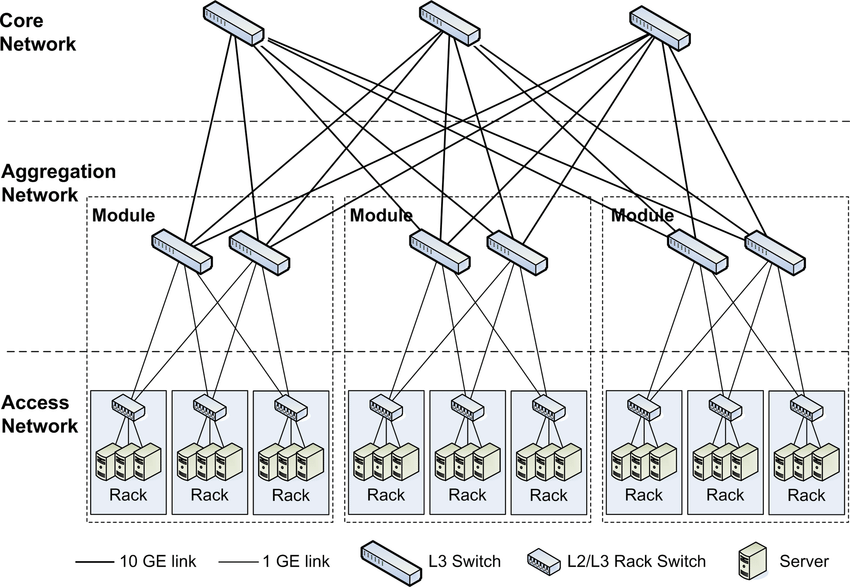
\includegraphics{images/3tier_switches.png}
      \caption{Three-tier architecture schema}
      \label{fig:3tier_switches}
   \end{figure}
   \colfill
   
\end{paracol}
This architecture is not used anymore, because it is not scalable, and it is not able to handle the high number of links and switches typical of a datacenter; more specifically, it does not fit virtualization most crucial need to be able to freely move VMs between servers.

\subsection{Spine Leaf architecture}
\begin{figure}[htbp]
   \centering
   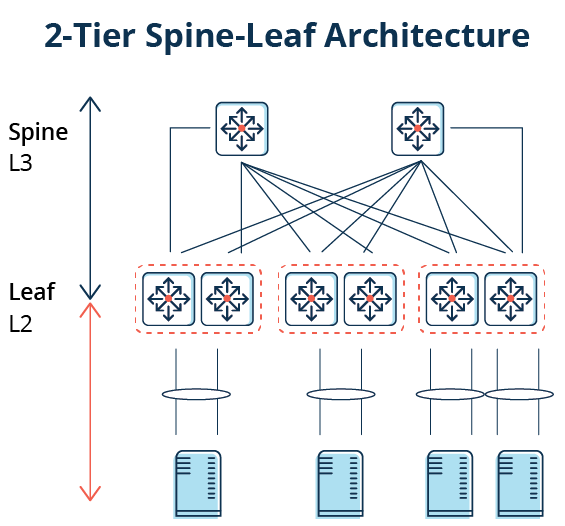
\includegraphics{images/spineleaf.png}
   \caption{Spine-leaf architecture schema (from \href{https://www.arubanetworks.com/faq/what-is-spine-leaf-architecture/}{Arubanetworks.com})}
   \label{fig:}
\end{figure}
A \textbf{spine-leaf} architecture is data center network topology that consists of two switching layers:
\begin{enumerate}
   \item \textbf{Spine layer}\\
   Swtiches responsible for routing traffic, working as the backbone of the network.   
   \item \textbf{Leaf layer}\\
   Switches connected to endpoints, such as servers, storage devices, firewalls, load balancers, edge routers, etc.
\end{enumerate}
Since \ul{every leaf switch is connected to every spine switch}, the spine-leaf architecture is a \textbf{fully connected} network,
ensuring that any source is always the same number of hops (actually only one \smiley) away from any destination, so latency is lower and predictable (fixed).

Capacity also improves because STP is no longer required. While STP enables redundant paths between two switches, only one can be active at any time. As a result, paths often become oversubscribed. 
Conversely, spine-leaf architectures rely on protocols such as \textit{Equal-Cost Multipath} (\texttt{ECMP}) routing to load balance traffic across all available paths while still preventing network loops.

Spine-leaf allows \textit{scale-out} opposed to \textit{scale-up}, by adding additional spine switches, ultimately increasing capacity in case the bandwidth is not enough; doing so reduces also the subscription

\subsubsection{LACP}
Loops are prevented using \texttt{LACP} (\textit{Link Aggregation Control Protocol}), which is a protocol that allows to aggregate multiple links into a single logical link, providing higher bandwidth and active-active redundancy (in case a link fails);
it also ensures no loops because each link is a single channel, and these are named \textit{port channels}.

LACP also provides a method to control the bundling of several physical ports together to form a single logical channel.

Note that even though the bandwidth is aggregated (i.e. $2\times 25Gbps$), the single stream is still limited to the bandwidth of a single link (i.e. $25Gbps$), because the traffic goes only from one way to the other each time.

\subsubsection{Advantages}

%TODO arrivato a pagina 27

\subsection{Full fat tree}
In a ---full?--- \textbf{fat tree}, branches nearer the top of the hierarchy are "fatter" (thicker) than branches further down the hierarchy. In a telecommunications network, the branches are data links; the varied thickness (bandwidth) of the data links allows for more efficient and technology-specific use.

Full-fat tree is rarely needed.

\section{Virtualization}

With VLAN frames are extended by 4 bytes. Every switch nowdays automatically sets the \texttt{VLAN\_ID} to \texttt{1}; if the field is not existent, it is appended, making an \textbf{tagged} an \textit{untagged} frame.

Switches ensure that data cannot spill/leak from a VLAN to another.
VLAN became largely of use when 10Gbit connection came out, because only 1Gbit was a too constrained bandwidth to be splitted into multiple VLANs. 

VLAN are used to partition the traffic at data link layer without having to redo the fabric. They are particularly useful in cloud environments.

\section{Network Administrator POV}
The switch is split in two planes:
\begin{itemize}
   \item \textbf{Control Plane}\\
   This plane is necessary to configure the data plane to make it behave according to our needs.
   Here there is an \textit{OS}, which used to be proprietary with a functioning fitting a specific network configuration, but nowdays they are usually more configurable and may even be \textit{open} OS.
   \note{\textit{Dell}'s switches now have an \textit{open} OS on board.}
   
   \item \textbf{Data Plane}\\
   Here lies the chip responsible to perform all the data link operations required, runs protocols, handles VLANs, etc.

   \textbf{OpenFlow} allows us to manage the flow table inside of a switch.
\end{itemize}

The two planes are linked by a low-bandwidth PCIe.


It is possible to use a very fast and simple ---reduced number of keystroke down to the strict necessary ones (e.g. \texttt{en} instead of \texttt{enable})--- CLI to program a switch. It is also possible to create a script file to be automatically executed by the switch at boot time.
\note{Prof. Cisternino performed a demo of this in class.}

Interestingly, the behaviour of the \texttt{netsh} command in Windows is very similar to the one of a switch.

\section{SDN}
\textbf{Software Defined Networking} is a new approach to networking that uses software-based controllers or application programming interfaces (APIs) to communicate with the underlying hardware infrastructure and direct traffic on the network.

The problem was that the network infrastructure was ``ossified'' and not programmable. SDN allows to program the network, and to make it more flexible and adaptable to the needs of the applications, without having to disrupt the existing infrastructure.

The key idea proposed in the OpenFlow article, which eventually became a standard, is to separate the control plane from the data plane, and to have a controller that can program through an API the data plane, where the \textbf{Flow Table} resides.

An interesting use of OpenFlow was implemented by a University and called Sandwich firewall, which consisted in routing the first part of the stream through a firewall and if the stream was not malicious, it was routed directly to the destination, otherwise it was dropped.

\subsection*{Latency-sensitive}
Some workloads are called \textit{latency-sensitive}, making the latency introduced by TCP-IP stack a problem.\\
Inside a datacenter nowadays the typical latency is sub microsecond.

Regarding this issue, technologies mentioned earlier come in handy; 
\textit{InfiniBand} is a fabric technology that allows to have a very low latency, and is used in HPC\footnote{High performance computing} environments, and \textit{OmniPath} is a technology that is similar to InfiniBand, but is more scalable and is its natural successor.
Also \textit{RDMA} and \textit{RoCE} are technologies that allow to access memory of a remote machine without involving the CPU or the OS of the remote machine, bypassing the TCP/IP stack.

\textit{Fibre Channel} switches are used in storage area networks, and are used to connect storage to servers CPUs. They are used in datacenters, but not for networking.